\documentclass[11pt]{article}
\usepackage[margin=1in]{geometry}
\usepackage{amsmath,amssymb,amsthm,mathtools}
\usepackage{booktabs,multirow}
\usepackage{microtype}
\usepackage{graphicx}
\usepackage{tikz}
\usetikzlibrary{arrows.meta,positioning,shapes.geometric}
\usepackage[numbers]{natbib}
\usepackage[hidelinks]{hyperref}
\usepackage{xcolor}
\usepackage{enumitem}
\usepackage{caption}
\usepackage{subcaption}
\usepackage{float}

\newtheorem{theorem}{Theorem}
\newtheorem{proposition}{Proposition}
\newtheorem{corollary}{Corollary}
\newtheorem{lemma}{Lemma}
\theoremstyle{remark}
\newtheorem{remark}{Remark}

\newcommand{\E}{\mathbb{E}}
\newcommand{\Pp}{\mathbb{P}}
\newcommand{\calV}{\mathcal{V}}
\newcommand{\calC}{\mathcal{C}}
\newcommand{\calH}{\mathcal{H}}
\newcommand{\tauR}{\tau_R}
\newcommand{\dtr}{\mathrm{DTR}}

\title{How Many Generations Are Enough?\\Adaptive Replication for Certified Diagnosis of Stochastic LLM Pipelines}
\author{Subir Hait\\Measurement and Quantitative Methods, Michigan State University}
\date{November 2026}

\begin{document}
\maketitle

\begin{abstract}
Repeated stochastic evaluation of large language model systems raises a budget-allocation problem: should every query receive the same number of generations? Uniform replication is wasteful when many query--regime pairs are nearly deterministic, yet reducing replication can weaken identification of nonlinear query-level response types. We introduce \emph{disagreement-triggered replication} (DTR), an adaptive design that begins each regime with two Bernoulli outcomes and continues to a maximum of $K$ only when the first two outcomes disagree. The main result is exact: the $K+1$ stopped-history likelihoods form a basis for the same degree-$K$ polynomial space identified by $K$ uniform replications. Tensoring across regimes therefore preserves the full finite-$K$ population identification used for certified component diagnosis. DTR uses only $2+2(K-2)p(1-p)$ expected generations for a query--regime pair with success probability $p$, implying at least a $(K-2)/(2K)$ expected saving relative to uniform $K$ for every latent distribution. Retrospectively applying DTR to ordered HotpotQA generations would have used 6,189 rather than 15,000 generations in the three diagnostic regimes, a 58.7\% saving. At nearly the same realized cost, however, exact projection intervals are wider than under uniform $K=2$, showing that identification preservation does not imply finite-sample efficiency. In a corner-concentrated simulation, reinvesting DTR's savings in additional queries reduces mean certified width by about 14\% relative to uniform $K=5$, and DTR eventually overtakes uniform $K=2$ as budget grows. The results turn ``how many generations?'' into an explicit identification--estimation design problem.
\end{abstract}

\section{Introduction}

Stochastic decoding makes repeated evaluation increasingly common in large language model (LLM) systems. A benchmark query may be generated several times to stabilize accuracy, estimate self-consistency, compare pipeline components, or diagnose whether retrieval or generation is the binding constraint. The default design is usually uniform: pick a replication count $K$ and run every query under every regime exactly $K$ times. That design is simple, but it can be expensive and statistically inefficient.

The waste is especially visible when repeated outcomes are concentrated near all-zero or all-one counts. In a companion analysis of retrieval-augmented generation (RAG), 95.9\% of the three-regime query--regime cells used for component diagnosis are observed at $0/5$ or $5/5$ \citep{Hait2026Partial}. Once two successive outcomes agree, spending three more generations on a cell that is almost deterministic may contribute little sampling information. At the same time, simply lowering $K$ is not innocuous: finite replication determines which polynomial functionals of the latent query-specific success probabilities are identified, and nonlinear response-type prevalences can remain partially identified even with infinitely many queries.

This paper asks a design question that is distinct from the identification question in the companion paper:
\begin{quote}
\emph{Given a limited generation budget, how should replications be allocated across query--regime cells while retaining certified population diagnosis?}
\end{quote}

We propose a particularly simple policy, \emph{disagreement-triggered replication} (DTR). For each query and regime, generate twice. If the two outcomes agree, stop that regime. If they disagree, continue until a prespecified maximum $K$. The rule uses only observed outcomes, needs no learned difficulty model, and has an exact algebraic property: its stopped-history likelihoods span the same polynomial space as the ordinary fixed-$K$ binomial counts. Thus DTR preserves the full finite-$K$ population identification while reducing expected generation cost.

This is an identification result, not a claim that the adaptive and fixed experiments have the same finite-sample information. Their multinomial laws have different covariance structures. The distinction appears in both simulation and real data. Retrospectively applying DTR to the ordered HotpotQA outputs from the companion experiment uses 6,189 generations across the three diagnostic regimes rather than 15,000, but at the same 1,000 queries its exact projection intervals are wider than those from uniform $K=5$. At nearly equal realized cost, uniform $K=2$ is also more precise under the conservative cellwise confidence construction. The value of adaptation appears when the saved generations are reinvested in more queries. In a HotpotQA-like corner-concentrated design, DTR with maximum $K=5$ uses about 6.13 generations per query across three regimes rather than 15. At an equal expected budget of 15,000 generations, this permits about 2,445 queries instead of 1,000 and reduces mean certified interval width by about 14\% relative to uniform $K=5$.

The budget trade-off is non-monotone. At the same 15,000-generation budget, uniform $K=2$ is even narrower because it spends the budget on more queries and estimates a much smaller count law, despite having a weaker population identification limit. But its interval cannot converge below the finite-$K=2$ population bracket. DTR retains the $K=5$ limit, so it eventually overtakes the coarse design. In a 60,000-generation simulation, DTR yields mean width .166 versus .178 for uniform $K=2$.

The contribution is complementary to recent work on adaptive LLM sampling. Adaptive self-consistency, early stopping, and test-time scaling allocate samples to improve answer quality or voting efficiency \citep{Kim2026ReASC,Na2026CASE,Wan2026BEACON,Nguyen2026UAB}. Factorized Active Querying adaptively chooses which benchmark questions to evaluate while maintaining confidence intervals for mean accuracy \citep{Wu2026FAQ}. ReliableEval studies how many prompt perturbations are needed for stable stochastic evaluation \citep{Lior2025ReliableEval}. Our target is different: we adapt \emph{within-query replication} while preserving identification of latent response-type prevalences under controlled component interventions.

The main contributions are:
\begin{enumerate}[leftmargin=*]
\item We prove that DTR identifies exactly the same coordinate-degree polynomial space as uniform $K$ replication.
\item We derive a distribution-free expected-cost bound: DTR uses at most $(K+2)/2$ expected generations per regime, versus $K$ under the fixed design.
\item We extend continuous-support certificate inference to the multinomial law of stopped histories, retaining finite-sample confidence transfer under i.i.d. query sampling.
\item We characterize the equal-budget trade-off between identification depth and query coverage, and demonstrate a budget crossover in a corner-concentrated RAG-like design.
\item We retrospectively apply DTR to the ordered HotpotQA replicate archive. It would have used 6,189 rather than 15,000 generations in the three diagnostic regimes, saving 58.7\%, and it exposes a real finite-sample trade-off against uniform $K=2$ and $K=5$.
\end{enumerate}

\section{Setup: response types under stochastic regimes}

Let $Q$ denote a query and let $j=1,\ldots,J$ index controlled pipeline regimes. Conditional on the query and a fixed system snapshot, regime $j$ has latent success probability
\[
 p_j(Q)=\Pp\{Y_{jk}(Q)=1\mid Q,j\},
\]
where repeated outcomes are conditionally i.i.d. Bernoulli. Regimes are run with separate random generation streams, so their histories are conditionally independent given the latent vector. Write $P=(p_1,\ldots,p_J)\sim F_P$ for the population distribution of query-specific success probabilities.

A component response type is a region $A\subseteq[0,1]^J$, with prevalence
\[
 \tau_A = \Pp(P\in A).
\]
For the three-regime RAG example $(p_{FF},p_{IF},p_{FI})$, retrieval-binding prevalence at threshold $\delta$ is
\[
 \tauR(\delta)=\Pp\{p_{IF}-p_{FF}>\delta,\;p_{FI}-p_{FF}\le\delta\}.
\]
With fixed $K$ replications per regime, the joint count law identifies the tensor polynomial space
\[
 \calV_K = \operatorname{span}\left\{\prod_{j=1}^Jp_j^{a_j}:0\le a_j\le K\right\},
\]
but not generally the full mixing distribution or a discontinuous response-region probability \citep{Hait2026Partial}. Continuous-support polynomial majorants and minorants convert this finite identified space into certified outer bounds.

The question here is whether the same population information can be obtained without always observing all $K$ outcomes.

\section{Disagreement-triggered replication}

\subsection{The design}

Fix a maximum replication level $K\ge3$. For each query--regime pair:
\begin{enumerate}[leftmargin=*]
\item Generate two Bernoulli outcomes.
\item If both are zero, stop and record history state $H=0$.
\item If both are one, stop and record $H=K$.
\item If they disagree, generate $K-2$ additional outcomes. If $d$ of those additional outcomes are successes, record $H=d+1\in\{1,\ldots,K-1\}$.
\end{enumerate}

Figure~\ref{fig:dtr} shows the rule for $K=5$.

\begin{figure}[H]
\centering
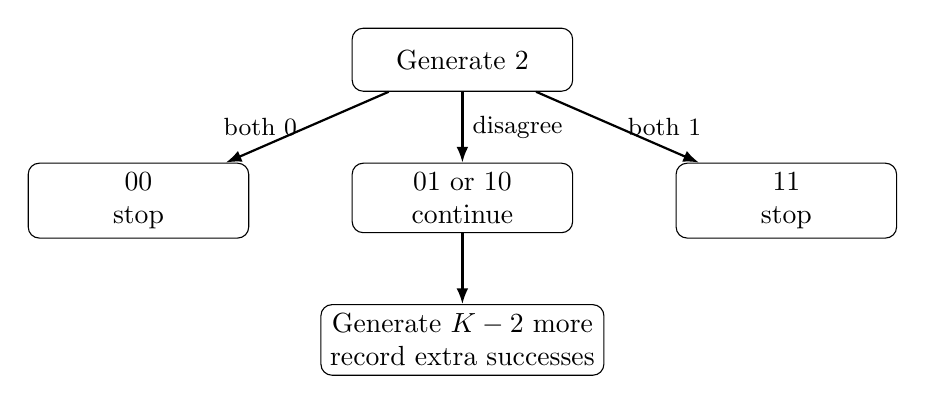
\begin{tikzpicture}[
node distance=9mm and 13mm,
box/.style={draw,rounded corners,minimum width=28mm,minimum height=8mm,align=center},
arr/.style={-{Latex[length=2mm]},thick}
]
\node[box] (start) {Generate 2};
\node[box,below left=of start] (agree0) {00\\stop};
\node[box,below=of start] (mixed) {01 or 10\\continue};
\node[box,below right=of start] (agree1) {11\\stop};
\node[box,below=of mixed] (extra) {Generate $K-2$ more\\record extra successes};
\draw[arr] (start)-- node[left,font=\small]{both 0} (agree0);
\draw[arr] (start)-- node[right,font=\small]{disagree} (mixed);
\draw[arr] (start)-- node[right,font=\small]{both 1} (agree1);
\draw[arr] (mixed)--(extra);
\end{tikzpicture}
\caption{Disagreement-triggered replication (DTR). The continuation decision is deterministic from the first two observed outcomes.}
\label{fig:dtr}
\end{figure}

For a single latent probability $p$, define the degree-$K$ Bernstein basis
\[
 b_{k,K}(p)={K\choose k}p^k(1-p)^{K-k},\qquad k=0,\ldots,K.
\]
The DTR history likelihoods are
\begin{align*}
 \psi_0(p)&=(1-p)^2,\\
 \psi_k(p)&=2{K-2\choose k-1}p^k(1-p)^{K-k},\qquad k=1,\ldots,K-1,\\
 \psi_K(p)&=p^2.
\end{align*}

\subsection{Identification preservation}

\begin{theorem}[DTR preserves the fixed-$K$ identified space]\label{thm:basis}
For every $K\ge3$, the $K+1$ DTR history likelihoods $\{\psi_0,\ldots,\psi_K\}$ form a basis of the univariate polynomial space of degree at most $K$. Consequently, if DTR is applied independently within each of $J$ regimes, the joint stopped-history law identifies exactly
\[
 \calV_K=\operatorname{span}\left\{\prod_{j=1}^Jp_j^{a_j}:0\le a_j\le K\right\},
\]
the same population polynomial space identified by uniform $K$ replication.
\end{theorem}

\begin{proof}
For $1\le k\le K-1$,
\[
 \psi_k(p)=\frac{2k(K-k)}{K(K-1)}\,b_{k,K}(p),
\]
so the interior Bernstein functions $b_{1,K},\ldots,b_{K-1,K}$ are directly recovered from the continuation-history likelihoods. Degree elevation gives
\[
 (1-p)^2=\sum_{k=0}^{K-2}\frac{(K-k)(K-k-1)}{K(K-1)}b_{k,K}(p),
\]
and
\[
 p^2=\sum_{k=2}^{K}\frac{k(k-1)}{K(K-1)}b_{k,K}(p).
\]
After recovering the interior Bernstein functions, the first equation uniquely isolates $b_{0,K}$ and the second uniquely isolates $b_{K,K}$. Hence the DTR likelihoods span the full degree-$K$ Bernstein basis and are linearly independent. Tensor products of bases are bases, yielding the result for $J$ regimes.\qedhere
\end{proof}

The theorem is a point-identification statement. It does \emph{not} say that one adaptive observation carries the same Fisher information as one complete fixed-$K$ count. The two multinomial experiments have different covariance structures, which matters for finite-sample precision.

\subsection{Generation cost}

Let $N_K(p)$ denote the number of generations used by DTR for one query--regime pair. Continuation occurs exactly when the first two outcomes disagree, which has probability $2p(1-p)$.

\begin{proposition}[Expected cost]\label{prop:cost}
Conditional on latent success probability $p$,
\[
 \E\{N_K(p)\}=2+2(K-2)p(1-p).
\]
Therefore
\[
 2\le \E\{N_K(p)\}\le \frac{K+2}{2},
\]
and DTR guarantees an expected fractional saving of at least
\[
 \frac{K-2}{2K}
\]
relative to uniform $K$ replication, for every latent distribution.
\end{proposition}

For $K=5$, the worst-case expected cost is $3.5$ generations per regime, a guaranteed 30\% saving. As $p\to0$ or $1$, expected cost approaches two, giving a 60\% saving.

For $J$ regimes with possibly different maxima $K_j$, independent regime-wise DTR identifies the tensor space with coordinate degrees $K_j$ and has expected total cost
\[
 \sum_{j=1}^J\left[2+2(K_j-2)\E\{p_j(1-p_j)\}\right].
\]

\section{Inference from stopped histories}

Let $H=(H_1,\ldots,H_J)\in\{0,\ldots,K\}^J$ denote the vector of DTR history states. Its population cell probabilities are
\[
 \eta_h=\E\left\{\prod_{j=1}^J\psi_{h_j}(p_j)\right\}.
\]
By Theorem~\ref{thm:basis}, $\eta$ is an invertible linear coordinate system for the same $\calV_K$ identified under uniform $K$ replication.

If a polynomial certificate $q(P)$ has degree-$K$ tensor Bernstein coefficients $\beta$, the basis transformation in Theorem~\ref{thm:basis} gives adaptive-history coefficients $\gamma$ such that
\[
 q(P)=\sum_h\gamma_h\prod_j\psi_{h_j}(p_j),
 \qquad
 \E q(P)=\gamma^\top\eta.
\]
Thus the continuous-support Bernstein--Handelman certificate program from the companion paper can be reused without changing its positivity constraints; only the coordinate representation of the expectation changes.

For $n$ i.i.d. queries, the stopped-history counts are multinomial with cell probabilities $\eta$. A simultaneous Clopper--Pearson box with Bonferroni allocation, intersected with the simplex, gives a finite-sample confidence region $\calC_n^\eta$. Confidence transfer then yields
\[
 U_n=\inf_{q\ge1_A}\sup_{\eta'\in\calC_n^\eta}\gamma(q)^\top\eta',
\]
with the analogous complement-majorant lower bound. The same single confidence region can be propagated to multiple response types and thresholds simultaneously.

A sharper count-law region is possible. KL concentration for empirical discrete distributions \citep{Mardia2020} is particularly attractive because DTR preserves the categorical alphabet size $(K+1)^J$ while often making the distribution sparse. Universal likelihood-ratio inference \citep{Wasserman2020} is another route for the mixture model. We leave those as extensions and use the transparent exact cellwise construction for the present design study.

\section{Equal-budget design}

Let $B$ denote the total generation budget across queries and regimes. A uniform design with replication level $k$ evaluates approximately
\[
 n_k(B)=\left\lfloor\frac{B}{Jk}\right\rfloor
\]
queries. DTR with maximum $K$ evaluates approximately
\[
 n_{\dtr}(B)=\left\lfloor\frac{B}{c_{\dtr}}\right\rfloor,
\]
where $c_{\dtr}$ is its expected generations per query.

Two effects compete. Lower fixed $k$ gives more queries and a lower-dimensional count law, but a weaker population identification limit. DTR has the same population limit as fixed $K$ but can estimate it from more queries per generation budget.

\begin{corollary}[Large-budget crossover]\label{cor:crossover}
Suppose confidence regions for each design contract to their population laws as $n\to\infty$, and let $W_D(B)$ denote the resulting certified interval width at budget $B$. DTR with maximum $K$ has the same limiting population width as uniform $K$. If that width is strictly smaller than the population width under a coarser uniform design $k<K$, then there exists a finite $B_0$ such that
\[
 W_{\dtr}(B)<W_k(B)
\]
for all sufficiently large $B>B_0$.
\end{corollary}

The corollary does not say where the crossover occurs. That is a finite-sample design question and depends on the latent distribution and the confidence construction.

\section{Simulation study}

\subsection{Corner-concentrated data-generating process}

We use the six-point three-regime distribution from the companion paper's HotpotQA-calibrated simulation. Let $\ell=.0075$ and $h=.9925$. The support points $(p_{FF},p_{IF},p_{FI})$ and weights are
\[
(\ell,\ell,\ell):.30,\quad
(h,h,h):.25,\quad
(\ell,h,\ell):.17,\quad
(h,\ell,h):.04,\quad
(\ell,\ell,h):.12,\quad
(\ell,h,h):.12.
\]
At threshold $\delta=.10$, true retrieval-binding prevalence is $.17$. With $K=5$, this design has the same qualitative corner concentration as the HotpotQA application.

The fixed-$K=5$ population certificate is $[.16875,.17401]$. By Theorem~\ref{thm:basis}, DTR with maximum five gives exactly the same population bracket; numerically the endpoints agree to solver precision.

Every coordinate of this DGP is either $\ell$ or $h$, so
\[
 p(1-p)=.00744375.
\]
DTR therefore uses
\[
 2+6p(1-p)=2.04466
\]
expected generations per regime, or $6.13399$ across the three regimes. Relative to uniform $K=5$, the expected saving is 59.1\%.

\subsection{Same queries versus same budget}

Table~\ref{tab:adaptive} reports a preliminary Monte Carlo study using exact Clopper--Pearson history regions. At the same $n=1000$ queries, DTR uses only about 6,132 generations instead of 15,000 but has a wider interval. When the saved budget is reinvested to evaluate about 2,445 queries, DTR becomes narrower than uniform $K=5$.

\begin{table}[H]
\centering
\caption{DTR versus uniform $K=5$ in the corner-concentrated design. Means over 20 replications.}
\label{tab:adaptive}
\begin{tabular}{lrrrr}
\toprule
Design & Queries & Mean budget & Mean interval & Mean width\\
\midrule
Uniform $K=5$ & 1000 & 15000 & $[.080,.528]$ & .448\\
DTR $2\to5$ & 1000 & 6132 & $[.018,.630]$ & .613\\
DTR $2\to5$, equal budget & 2445 & 14993 & $[.079,.464]$ & .385\\
\bottomrule
\end{tabular}
\end{table}

At equal budget, DTR reduces mean width by approximately 14\% relative to uniform $K=5$. All intervals covered the true value in these preliminary replications; the simulation is intended to compare width, not to estimate coverage precisely.

\subsection{The best fixed replication level can be smaller}

The adaptive design does not dominate every uniform design at every budget. Table~\ref{tab:fixedbudget} allocates approximately 15,000 generations across fixed replication levels. The coarsest design, $K=2$, is narrowest at this moderate budget because it evaluates 2,500 queries and has only $3^3=27$ count cells.

\begin{table}[H]
\centering
\caption{Equal-budget comparison at about 15,000 generations. Fixed designs use 20 Monte Carlo replications; DTR uses 20 independent replications.}
\label{tab:fixedbudget}
\begin{tabular}{lrrr}
\toprule
Design & Queries & Population width & Mean confidence width\\
\midrule
Uniform $K=2$ & 2500 & .0924 & .289\\
Uniform $K=3$ & 1666 & .0649 & .344\\
Uniform $K=4$ & 1250 & .0075 & .408\\
Uniform $K=5$ & 1000 & .0053 & .456\\
DTR $2\to5$ & 2445 & .0053 & .385\\
\bottomrule
\end{tabular}
\end{table}

This table is the central design trade-off. At small and moderate budgets, sampling more queries at low $K$ can outweigh the loss in population identification. But the low-$K$ interval has a nonzero limiting width. DTR keeps the $K=5$ limit while spending far less per query.

\subsection{Budget crossover}

Figure~\ref{fig:budget} plots a planning curve obtained by holding the population history geometry fixed and shrinking exact count-cell confidence regions with hypothetical budget. It is not a Monte Carlo result, but it reveals the crossover. DTR is worse than uniform $K=2$ at 15,000 generations, approximately tied near 60,000, and better thereafter.

\begin{figure}[H]
\centering
\includegraphics[width=.84\textwidth]{budget_curve.png}
\caption{Plug-in planning curve under the corner-concentrated population geometry. The curve isolates how confidence-region contraction interacts with each design; it is not a Monte Carlo average.}
\label{fig:budget}
\end{figure}

A direct 10-replication Monte Carlo check at $B=60{,}000$ confirms the crossover: DTR has mean interval $[.131,.297]$ with width .166, compared with $[.123,.300]$ and width .178 for uniform $K=2$.

\section{Retrospective HotpotQA experiment}

The companion RAG experiment records the replicate order, random seed, regime, and exact-match outcome for all generations \citep{Hait2026Partial}. We therefore applied DTR retrospectively to the first two outcomes of each of the 3,000 query--regime cells used for response-type diagnosis. A cell stops after two outcomes when they agree; otherwise the recorded third through fifth outcomes are retained.

DTR stops 2,937 of the 3,000 cells (97.9\%) after two draws. The stop rates are 97.8\% in FF, 97.3\% in IF, and 98.6\% in FI. Only 63 cells continue to five draws. At the query level, 942 of 1,000 queries use exactly six generations across the three regimes, 53 use nine, and five use twelve; none requires all fifteen. The realized DTR budget is therefore
\[
 6189
\]
generations, compared with 15,000 for uniform $K=5$: a saving of 8,811 generations, or 58.74\%. The adaptive joint-history distribution occupies 42 of its 216 possible cells.

Because the stopped histories form the same degree-five identified polynomial space as fixed $K=5$, we can recompute the certified response-type intervals using the exact simultaneous Clopper--Pearson region on adaptive history probabilities. Table~\ref{tab:hotpotreal} compares DTR with two fixed designs. Uniform $K=2$ uses only the first two recorded outcomes in every regime and therefore costs 6,000 generations, almost exactly the DTR budget. Uniform $K=5$ is the published companion-paper analysis.

\begin{table}[H]
\centering
\caption{Real HotpotQA retrospective comparison at $\delta=.10$. All intervals use exact Bonferroni--Clopper--Pearson projection in their native observable coordinates.}
\label{tab:hotpotreal}
\begin{tabular}{lrrrr}
\toprule
Design & Generations & Retrieval-binding & Generation-binding & Retrieval-harm\\
\midrule
Uniform $K=2$ & 6000 & $[.047,.539]$ & $[.025,.514]$ & $[.009,.497]$\\
DTR $2\to5$ & 6189 & $[.008,.575]$ & $[0,.595]$ & $[0,.613]$\\
Uniform $K=5$ & 15000 & $[.064,.469]$ & $[.053,.478]$ & $[.013,.428]$\\
\bottomrule
\end{tabular}
\end{table}

The result is intentionally not a dominance claim. DTR preserves the $K=5$ \emph{population} identified space while using nearly the same realized budget as uniform $K=2$, but the conservative cellwise confidence region is less efficient for the 216 adaptive-history probabilities than for the 27 $K=2$ count cells. At $n=1000$, the near-equal-cost $K=2$ intervals are therefore shorter. Uniform $K=5$ is shorter still for some targets because it spends more than twice the generations. This real-data comparison mirrors the simulation: adaptation creates compute savings, but those savings become statistically valuable only when they are reinvested in additional queries or paired with a sharper confidence region.

\section{Related adaptive LLM evaluation}

Several recent methods allocate inference compute adaptively. Reliability-Aware Adaptive Self-Consistency and confidence-aware early stopping reduce self-consistency sampling \citep{Kim2026ReASC,Na2026CASE}; BEACON uses Bayesian optimal stopping to trade response quality against cost \citep{Wan2026BEACON}; and uncertainty-aware budget allocation distributes test-time reasoning samples according to query uncertainty \citep{Nguyen2026UAB}. These methods optimize the quality or efficiency of the \emph{generated answer}. DTR instead targets the statistical information retained by an \emph{evaluation experiment}.

A closer evaluation contribution is Factorized Active Querying, which adaptively selects benchmark questions while maintaining confidence intervals for mean model accuracy \citep{Wu2026FAQ}. DTR operates on the orthogonal axis: which repeated outcomes to collect within an already selected query. ReliableEval studies stochastic prompt resampling and estimates how many perturbations are required for stable evaluation \citep{Lior2025ReliableEval}. Our target is nonlinear population heterogeneity across controlled regimes rather than a stable mean score.

These distinctions suggest a broader design space. Query selection and within-query replication can be combined: an outer active design chooses questions, while an inner DTR-like design chooses replications. The resulting stopped-history likelihood remains known when both selection mechanisms are recorded, but valid population inference then depends on the query-sampling design as well as the within-query stopping rule.

\section{Discussion}

The main lesson is that preserving \emph{identification} and preserving \emph{precision} are different objectives. DTR is identification-preserving in a strong algebraic sense: it spans the same $\calV_K$ as fixed $K$. Yet at equal $n$ its confidence intervals are wider because the adaptive history probabilities encode the same polynomial information with different sampling variance. The savings become useful when they purchase more queries.

This creates an identification--estimation frontier. Small fixed $K$ is attractive at low budgets because it maximizes query coverage and minimizes categorical dimension. Large fixed $K$ has the strongest population limit but may spend heavily on nearly deterministic cells. DTR occupies a third point: it inherits the large-$K$ population limit while making its average cost depend on latent uncertainty $p(1-p)$. Corner concentration is therefore not merely a descriptive feature; it is a resource that an adaptive design can exploit.

The present rule is intentionally simple. It treats each regime independently and uses disagreement of two outcomes as the sole continuation trigger. More aggressive policies could condition on the full cross-regime state, current certificate sensitivity, query covariates, or estimated contribution to interval width. Those policies need not preserve $\calV_K$ automatically. Theorem~\ref{thm:basis} provides a benchmark: any more complicated adaptive rule should be compared against a design that already saves substantial compute without sacrificing the fixed-$K$ identified space.

Sharper inference is another priority. Bonferroni--Clopper--Pearson projection is exact but conservative for a large sparse alphabet. KL balls for multinomial laws \citep{Mardia2020} and split likelihood-ratio methods \citep{Wasserman2020} could reduce this cost and may move the budget crossover substantially downward.

\section{Limitations and next empirical step}

The real HotpotQA experiment establishes realized compute savings and the finite-sample trade-off using the existing $K=5$ archive, but it cannot validate low-replication diagnoses against near-true query probabilities. The most important next experiment is therefore a high-replication reference panel: run 200--300 queries at $K=50$--100 under several regimes, treat the resulting high-replication intervals as a reference rather than literal ground truth, and compare fixed and adaptive designs on the same realized LLM outputs.

The current finite-sample guarantee assumes i.i.d. query sampling from a superpopulation. Fixed benchmark inference requires a design-valid finite-population region. The Bernoulli-with-stable-$p$ model also assumes a fixed system snapshot and conditionally i.i.d. decoding within a query--regime pair. Provider drift, hidden state, or correlated sampling can violate that model.

Finally, DTR assumes binary outcomes. Extensions to multinomial labels, continuous scores, and semantic-judge outputs require different history bases. The identification-preserving principle suggests a general question: can one construct stopped likelihood histories that form a basis for the same finite-dimensional experiment as a fixed sampling design while reducing expected cost?

\section{Conclusion}

Uniform stochastic replication is not the only way to obtain high-$K$ population identification. A two-stage rule that continues only after initial disagreement preserves the entire degree-$K$ polynomial space while using fewer generations for every latent distribution. In the recorded HotpotQA experiment, the rule would have saved 58.7\% of the three-regime generation budget. Yet the real-data confidence intervals also show why compute saving alone is not enough: under conservative cellwise inference, a nearly equal-cost uniform $K=2$ design is more precise at $n=1000$. The resulting design problem is therefore genuinely two-dimensional. Coarse fixed replication can be preferable at small budgets, while identification-preserving adaptation becomes more attractive when saved generations can purchase additional queries or when sharper confidence regions are available. Replication count should be treated as an explicit statistical design choice rather than a fixed benchmark convention.

\appendix
\section{Linear transformation between fixed counts and DTR histories}

Let $A_K$ be the $(K+1)\times(K+1)$ matrix such that
\[
 \psi_h(p)=\sum_{k=0}^K (A_K)_{hk}b_{k,K}(p).
\]
The nonzero entries are
\begin{align*}
(A_K)_{0k}&=\frac{(K-k)(K-k-1)}{K(K-1)}, &&0\le k\le K-2,\\
(A_K)_{kk}&=\frac{2k(K-k)}{K(K-1)}, &&1\le k\le K-1,\\
(A_K)_{Kk}&=\frac{k(k-1)}{K(K-1)}, &&2\le k\le K.
\end{align*}
The proof of Theorem~\ref{thm:basis} shows $A_K$ is nonsingular. For $J$ regimes, the adaptive history law $\eta$ and fixed-$K$ count law $\pi$ satisfy
\[
 \eta=A_K^{\otimes J}\pi.
\]
Thus the two population coordinate systems are related by an invertible linear map on the identified polynomial space. This is the transformation used in the adaptive certificate computations.

\bibliographystyle{plainnat}
\bibliography{references}
\end{document}